%**************** SoTA **************

\chapter{State of the Art}
\label{chapter:sota}
As presented in the introductory chapter, this dissertation focuses on two main applications: automatic transcription and spoken language translation. In the first part of this chapter, I will give an overview on the main research areas that are related to these two topics with a focus on neural network-based approaches. Automatic transcription, which is made possible with \textit{automatic speech recognition (ASR)}, is explained in Section \ref{sota:asr}. Approaches to the task of punctuation recovery in ASR output are presented in Section \ref{sota:punk_on_asr}. \textit{Neural machine translation} is presented in Section \ref{sota:nmt} with a focus on \textit{spoken language machine translation}. After a brief introduction to text-to-speech synthesis (TTS) systems in Section \ref{sota:tts}, I will present the concept of speech-to-speech translation with recent work on its field in Section \ref{sota:s2s}. Next, in Section \ref{sota:prosody}, I will give an overview on Prosody. Finally, the last part of this chapter reviews relevant work on the inclusion of prosody into these systems. Focus is given on usage of prosody in punctuation recovery in Section \ref{sota:punk_prosody} and adding prosodic modelling on spoken language translation in Section \ref{sota:prosody_in_smt}. 


\section{Neural Speech Processing Overview}
\label{sota:neuralspeech}
%speech processing systems overview

A spoken language system consists of at least one of the following modules: automatic Speech Recognition (ASR) for converting verbal communication into discrete symbolic form (i.e.~text), text-to-speech (TTS) system for generating information in spoken form, and a spoken language understanding (SLU) system for mapping between actions and verbal utterances \citep{slp_book}. Depending on the application, versions and combinations of these systems are employed to solve the task involved with it. For instance, an automatic subtitling system would involve an ASR system together with a speech activity detection module to transcribe the spoken parts in a media. If the subtitling is to be done in another language, the same pipeline would be followed by a machine translation system. A complete speech-to-speech pipeline would result in an automatic dubbing system where translated content would be synthesized using a TTS system. 

%neural networks overview. 
Research on these subareas of speech technology has recently experienced a great shift towards the usage of \textit{artificial neural networks (ANN)}. Popularity of ANN in general has risen in the recent years mostly due to advancements in computing power. Specifically, training of large and deep neural networks (DNN) in a reasonable amount of time has been made possible with \textit{Graphical Processing Units (GPUs)}.

I will introduce briefly the concept of DNNs as they form the basis of the experimentation presented in this dissertation. The information presented in this section can be consulted in \cite{shigeru2000handbook} and \cite{bengio_dl} for a \textit{deeper} understanding. 

\subsection{Deep Neural Networks}
\label{sota:dnns}

\begin{figure}[t]
  \centering
  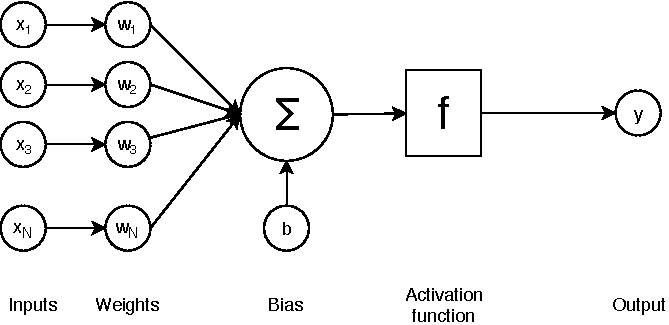
\includegraphics[width=0.6\linewidth]{img/perceptron.pdf}
  \caption{An artificial neuron.}
  \label{sota:neuron}
\end{figure}

An artificial neural network consists of a group of nodes and connections between them, inspired respectively by the neurons and axons in a biological neural system. Figure \ref{sota:neuron} illustrates the structure of one neural node, which is also referred as \textit{perceptron} or simply \textit{neuron}. Each connection towards a neuron is an input ($x_i$) and is associated with a weight coefficient ($w_i$). The basic function of a neuron defines the input signal to the neuron as:
\begin{equation}
    a = \sum _{ i }{ w_i x_i + b} 
\end{equation}

The input signal is then passed into an activation function to produce the output $y$. 

\begin{equation}
    y = f(a)
\end{equation}

Activation function is a differentiable function that originally resembles a step function so that the neuron \textit{fires} with certain input. The original Rosenblatt's perceptron had Heaviside step function as the activation function \citep{Rosenblatt58theperceptron}. Activation functions commonly being used today are the \textit{sigmoid} and the \textit{hyperbolic tangent} functions. 

One single neuron is evidently not sufficient for modelling complex functions. A basic neural network consists of a layer of input neurons fully connected to a layer of output neurons. This setting produces an N-to-M mapping. Extra layers are added between the input and output layers to introduce even more complexity to the network. These layers are called \textit{hidden layers} and are fully connected between each other between input and output layers. An illustration of a neural network with two hidden layers is given in Figure \ref{sota:neuralnet}. Number of hidden layers can be determined according to the task-at-hand. A neural network with more than one hidden layer is called a \textit{deep neural network} \citep{yoav}. 

\begin{figure}[t]
  \centering
  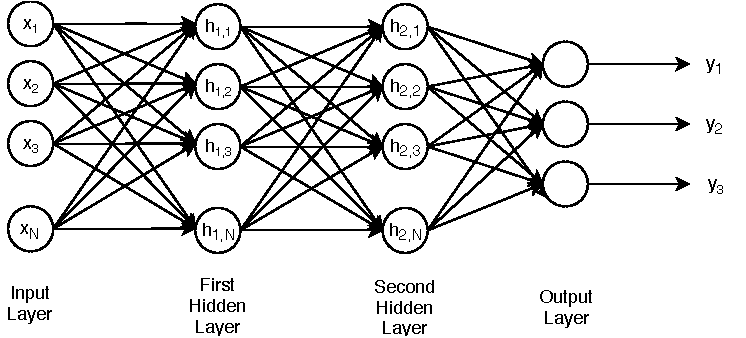
\includegraphics[width=0.9\linewidth]{img/NeuralNet.pdf}
  \caption{A fully connected feed-forward neural network with two hidden layers.}
  \label{sota:neuralnet}
\end{figure}

Although there exist many types of neural network taxonomies, one important characteristic that divides neural network architectures into two is the direction of the signal flow in the network. A \textit{feed-forward} network (as in the example in Figure \ref{sota:neuralnet}) allows information to be passed only in one direction, whereas a \textit{recurrent neural network (RNN)} network allows the output signal of some nodes to be passed again to a neuron coming previously, or to the neuron itself. Recurrent neural networks are especially suitable for representing time-series data. Because of this, it is currently being preferred as the principal architecture in many state-of-the-art applications of machine translation, speech recognition and speech synthesis. 

\begin{figure}[t]
  \centering
  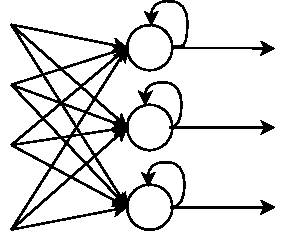
\includegraphics[width=0.3\linewidth]{img/RecurrentNeuralNet.pdf}
  \caption[Information flow in a recurrent neural network (RNN).]{Information flow in a recurrent neural network (RNN). Output signals are allowed to go back as input signals to the neurons. }
  \label{sota:rnn}
\end{figure}

As it can be seen in Figure \ref{sota:rnn}, a neuron in a RNN can have its output connected back to itself as an input. This model allows the neuron to keep a form of a \textit{memory} from previous inputs and decide on the next output according to it together with the current input. Modelling inputs and outputs in a time-series enables the processing of either a fixed number or a sequence of vectors, one at a time. Different types of RNN-based architectures is demonstrated in Figure \ref{sota:rnn_connections}. A one-to-one network serves for fixed size input and output at each time step. Although this architecture is useful in, for example, image classification, it is not sufficient for modelling variable length data. A ``many'' type input or output means an arbitrary number of vectors can be introduced to and/or obtained from the model at each time step. Many-to-many architecture can either have input and output sequences synchronized (left in the figure), where an output is given for each input vector, or not (right in the figure). An example to an non-synchronized many-to-many type architecture is machine translation. A sequence of vectors representing words in source sentence is first input to the model. Then, words from the translated sentence are decoded from the output layer. This group of neural networks are sometimes called \textit{encoder-decoder networks}. Many-to-many type RNN is sometimes referred to as a \textit{sequence-to-sequence network} as introduced in \cite{sutskever}. 

\begin{figure}[t]
  \centering
  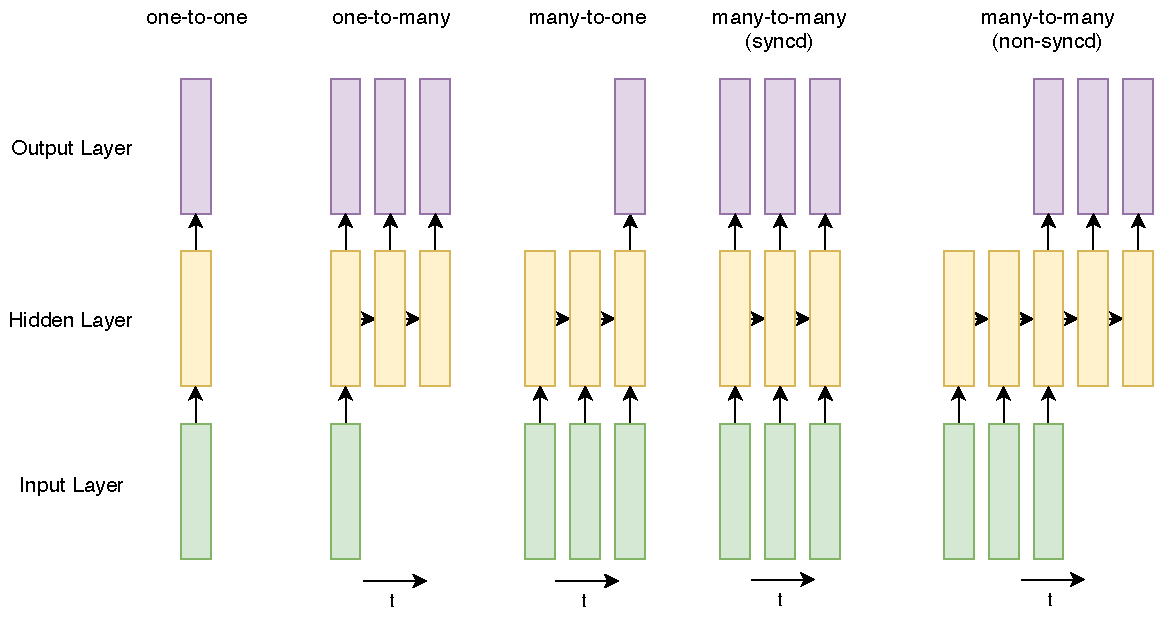
\includegraphics[width=\linewidth]{img/rnn_types.pdf}
  \caption[Various types of RNN architectures.]{Various types of RNN architectures. Each box represents a vector. }
  \label{sota:rnn_connections}
\end{figure}

%backpropagation
\subsubsection*{Neural Network Training}
The steps involved in neural network training can be summarized as follows: (1) introduction of samples in the training set to the network, (2) computing the error of the network regarding the desired and obtained output from the network, (3) computing the gradient given by the error and then (4) moving the network weights in the direction and magnitude of the gradient. 

The error of a network is calculated with the \textit{loss function}:

\begin{equation}
    E = \frac { 1 } { 2 } \left( y - f \left( \sum w _ { i } x _ { i } \right) \right) ^ { 2 }
\end{equation}

where $y$ represents the desired output, and $f(x)$ giving the output of the neural network. Using a method called \textit{backpropagation}, the error given by this function is traced back in the network layers using reverse differentiation. This is done by calculating the gradient of the loss function $\nabla J ( \theta )$ with respect to the weights $ \theta $ of the network.

Updating of the weights of the network is done with an \textit{optimization algorithm}. The \textit{gradient descent} technique is used to find the minima in an error space by updating the parameters of the network in the opposite direction of the gradient scaled with a learning rate $\eta$:

\begin{equation}
 \theta =  \theta -  \eta \cdot \nabla J(  \theta )
\end{equation}

As the calculation of loss with respect to the whole dataset would be cumbersome for large training sets, \textit{stochastic gradient descent (SGD)} \citep{bengio_dl, sgd2} does the parameter updates for each training sample $\{ x ( i ) , y ( i ) \}$:

\begin{equation}
    \theta = \theta -  \eta \cdot  \nabla J ( \theta  ;  x ( i  ) ;  y  ( i ) )
\end{equation}

However, this method causes unnecessary fluctuations (i.e.~noise) in weight updates as it is done at each input sample. To avoid this, samples are input in batches and the average loss for that batch is used to update the network instead.

Learning rate $\eta$ is a key hyperparameter in setting up neural network training. Optimization on the selection and variance of this parameter is often crucial in DNN architectures. \textit{Learning rate scheduling} is performed to help network converge with smaller updates through the later stages of training. Several variations on the SGD account for this aspect and further adapts the learning rate at each batch to each parameter. \textit{Adagrad} does this modification based on past gradients that were calculated for the parameters \citep{adagrad}. \textit{Adam} chooses an accelarated learning rate in relavant directions and diminishes it in irrelevant directions \citep{DBLP:journals/corr/KingmaB14}. 

\subsubsection*{Addressing the Problems of RNN}
There is a number of issues that has emerged in the development of RNNs and much of it is addressed in various works. First one is the issue that is common in any machine learning problem, which is \textit{overfitting}. A model is said to overfit on training data when it covers too well noisy data inside it and fails to generalize on anything outside it. Overfitting can be avoided by applying regularization techniques such as \textit{dropout} \citep{dropout}. This particular technique functions by randomly deactivating a portion of a layer's weights at each pass of a training sample, so that the network does not end up relying on specific weights \citep{bengio_dl}.

Two problems specific to the training of RNNs are \textit{exploding and vanishing gradients}. It is common that gradients end up either growing extremely high or extremely low during the course of backpropagation. The issue of exploding gradients is simply solved by putting a threshold on the magnitude of the gradients, and \textit{clipping} it once it is exceeded. On the other hand, resolution of vanishing gradient is still seen as an open research problem. Both these problems contribute to the shortcoming of RNNs in remembering long-term dependencies. \cite{longterm_is_difficult:1994} explores this issue in deep and stated the inefficiency of the gradient descent algorithm especially in preserving gradients across longer sequences. 

The issue with the short-term memory in RNNs was addressed with the introduction of \textit{Long-Short Term Memory (LSTM)} \citep{lstms}. LSTM defined a mechanism of \textit{gates} which decides on the information flow at each time-step. Gates decide which information is allowed to pass by through \textit{input} and \textit{output} gates, and which are bound to be discarded with the \textit{forget} gates. Although LSTM was an efficient solution for modelling long-term dependencies, it was also a complicated one \citep{bengio_dl}. Gated recurrent unit (GRU), was introduced as a simpler variant of LSTM units and made computation simpler by having fewer parameters \cite{gru}. Number of gates were reduced to two where the \textit{reset} gate determined whether the previous memory will be ignored, and the \textit{update} gate determines how much of the previous memory will be carried on. An illustration of architectures of both LSTM and GRU cells is given in Figure \ref{sota:figure:lstm_gru}.

\begin{figure}[t]
  \centering
  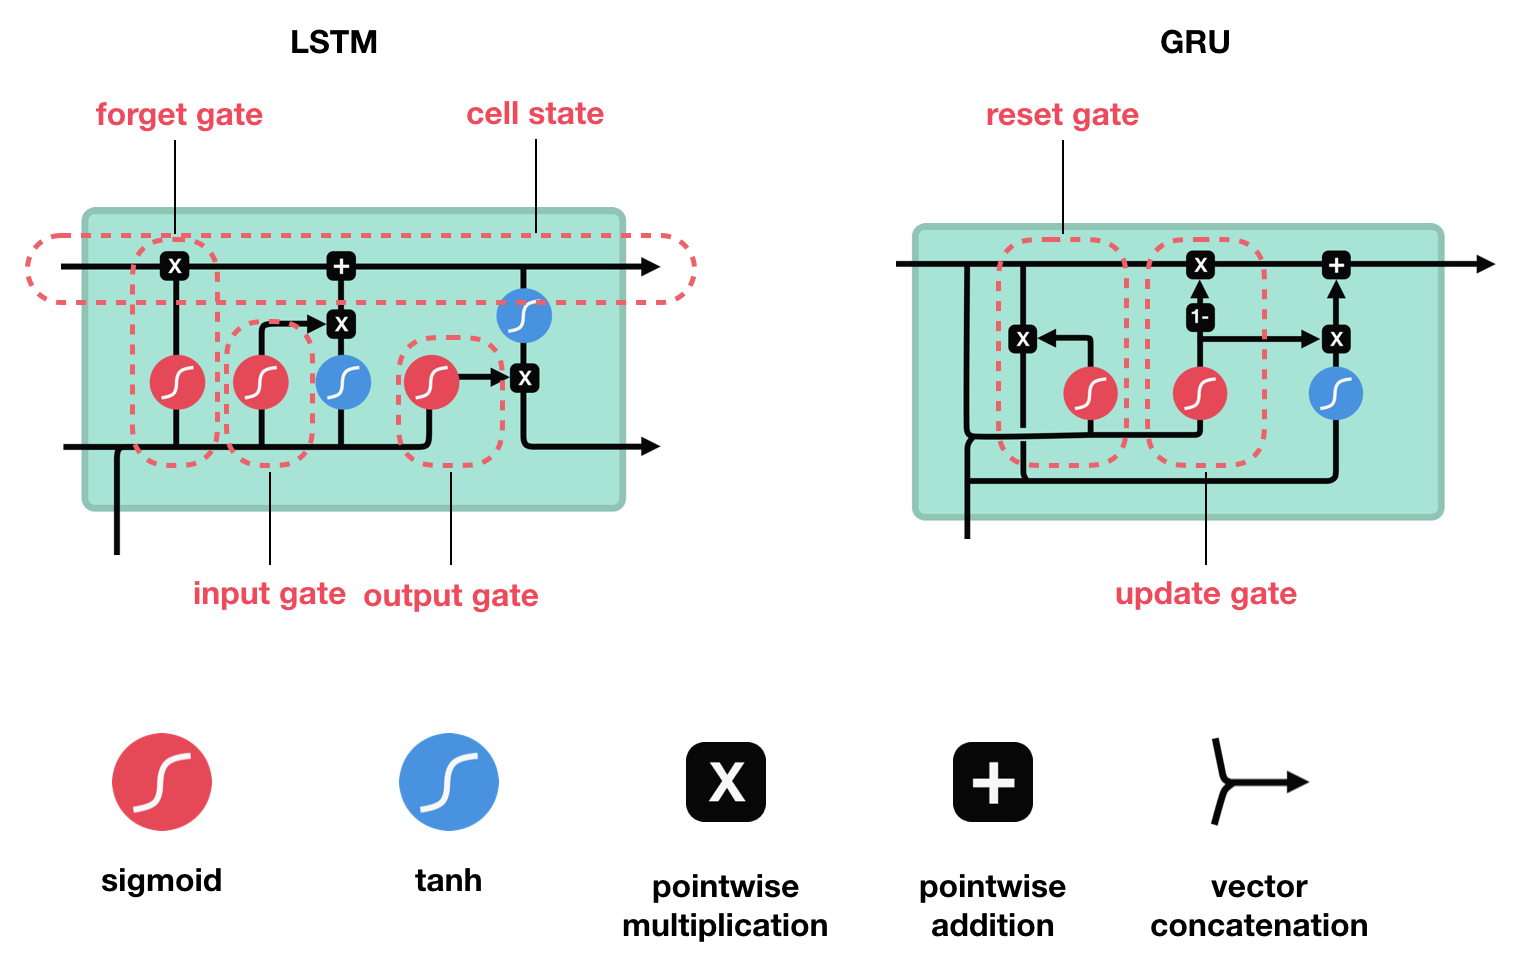
\includegraphics[width=0.85\linewidth]{img/lstm_gru.png}
  \caption[Architectures of a LSTM and GRU cell.]{Architectures of a LSTM and GRU cell. (Diagram from Michael Nguyen's article on Medium\protect\footnotemark)}
  \label{sota:figure:lstm_gru}
\end{figure}

\footnotetext{\url{https://towardsdatascience.com/illustrated-guide-to-lstms-and-} \url{gru-s-a-step-by-step-explanation-44e9eb85bf21}}

\subsection{Automatic Speech Recognition}
\label{sota:asr}

In its most simple sense, automatic speech recognition (ASR) is the conversion of speech in its acoustic form into a symbolic form such as words or letters. It is the probabilistic modelling of the question "What is the most probable word sequence among all possible word sequences given an acoustic input?". Figure \ref{sota:asr_process} illustrates this process. Speech signal captured by a microphone is first encoded into a sequence of acoustic feature vectors. Following, the acoustic feature vectors are decoded into the words that represent the linguistic information that lies in the speech signal. 

\begin{figure}[t]
  \centering
  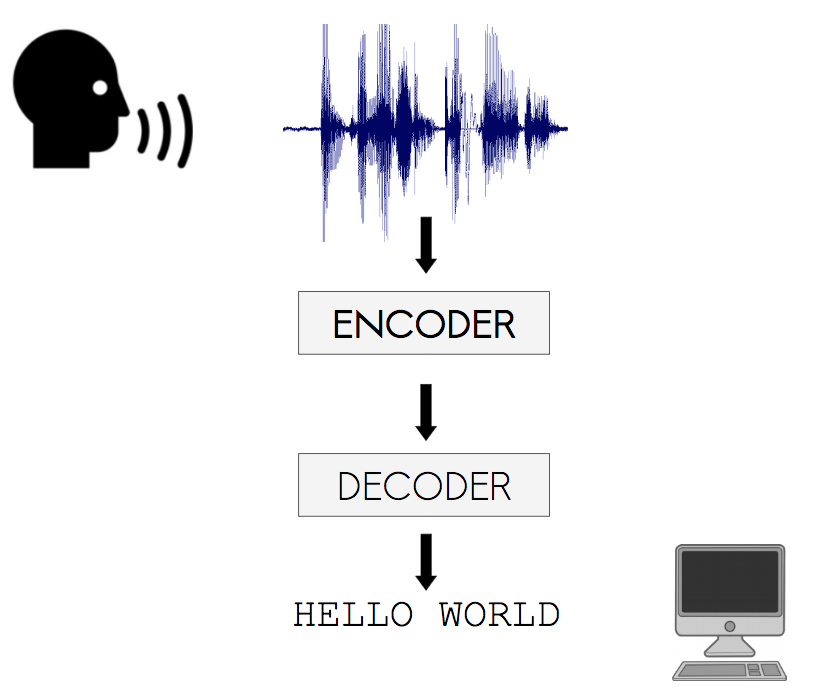
\includegraphics[width=0.5\linewidth]{img/asr_schema.png}
  \caption[Speech recognition.]{Speech recognition is the conversion of an acoustic signal with spoken language into its written form. }
  \label{sota:asr_process}
\end{figure}

Classical approaches to ASR employ a modeling of spoken language that uses Gaussian mixture model-hidden Markov model (GMM-HMM). HMM is a powerful statistical method for representing time-series data \citep{slp_book, hmm_balls}. As illustrated in Figure \ref{sota:asr_schema}, a GMM-HMM ASR system has a modular architecture: The feature extraction step converts the input speech signal into a sequence of fixed size acoustic vectors. Later, the decoder makes use of the acoustic model, the language model and the pronunciation dictionary in order to decide the most likely word sequences they represent. Acoustic and language models are trained with a corpus of transcribed speech samples and a text corpus respectively. While the acoustic model stores the information of the statistical behaviour of the sounds in a language, the language model stores the likelihood of the tokens (words) occurring and co-occurring in a language. 

\begin{figure}[t]
  \centering
  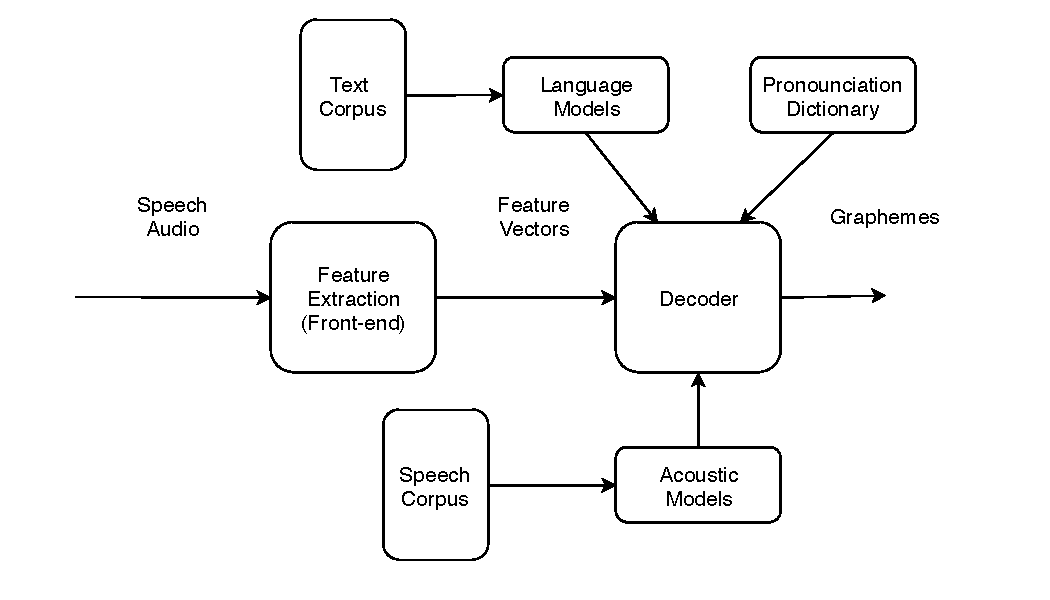
\includegraphics[width=0.8\linewidth]{img/asr2.pdf}
  \caption{General architecture of a traditional ASR system.}
  \label{sota:asr_schema}
\end{figure}

ASR systems experienced a breakthrough with the use of deep neural networks from 2012 on with its introduction in \cite{asr_dnnhmm}. The hybrid DNN-HMM model replaced the feature representation step that used Gaussian mixtures with a RNN-based architecture. The graphical comparison of the acoustic modelling of the two models is illustrated in Figure \ref{sota:gmm-dnn-hmm}. The DNN-HMM based ASR showed an improvement of 20\% in sentence accuracy compared to the GMM-HMM based model in a large-vocabulary task. 

\begin{figure}
\begin{tabular}{cc}
  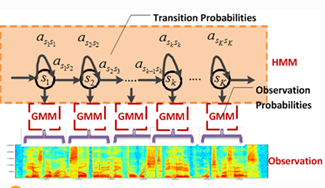
\includegraphics[width=0.5\linewidth]{img/gmm-hmm.png} &   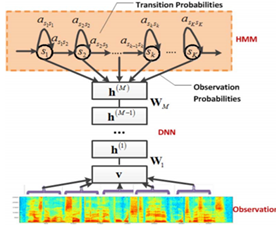
\includegraphics[width=0.5\linewidth]{img/dnn-hmm.png} \\
(a) GMM-HMM & (b) DNN-HMM\\[6pt]
\end{tabular}
\caption[Comparison between GMM based and DNN based ASR.]{Comparison between GMM based (a) and DNN based (b) ASR (Figure from \cite{asr_dnnhmm})}
\label{sota:gmm-dnn-hmm}
\end{figure}

More recently, end-to-end systems were introduced that made large-vocabulary speech recognition possible even without a language model or a lexicon \citep{e2e_asr}. Graves and Jaitly suggested a model that maps directly between spectral features and characters using a deep bidirectional LSTM and Connectionist Temporal Classification \citep{Graves:ctc} as loss function. Although this approach did not beat the hybrid approach baseline, it was a breakthrough for remedying a complex modular architecture that depended on separate acoustic, phonetic and language modelling. Later advancements, however, report outperforming of the hybrid methods both in terms of recognition accuracy and noise robustness \citep{deepspeech}.

\subsection{Punctuation Restoration in ASR Generated Transcripts}
\label{sota:punk_on_asr}

As applications of automatic speech recognition vary greatly, the objective of ASR is only focused on the recognition rate of the words. Aspects such as capitalization and punctuation, which are crucial elements for readability of the ASR output, is generally considered apart from an ASR system. For applications such as automatic captioning or transcript extraction, punctuation and capitalization prove to be essential for improving readability. In broadcast domain, \cite{Tundik2018} evaluate the effect of presence of punctuation in captions from an end-user perspective and show that punctuated captions are easier to read both when transcriptions are manually or automatically generated. In clinical domain, \cite{emrai} points out the importance of punctuation in the reports dictated by medical doctors. 

Another case where punctuation proves to be essential is when subsequent processing steps in spoken language system pipeline are optimized to work with it. Syntactic or semantic parsing, which is an important module in dialog based systems, necessitates input segmented into sentence-like units to function. Most machine translation systems are trained with single sentence input \citep{niehues2018}. Furthermore, it is proved that both of these processes function better with properly placed in-sentence punctuation and especially commas \citep{10045_76089, Jones:1994:ERP:991886.991960}. 

%from CSL
% TEXT
The problem of punctuation restoration has been addressed in several works in the literature --as has been the closely-related issue of boundary detection. Both problems have been tackled from diverse perspectives. In terms of which types of features are used, the approaches fall into three categories: (1) models based only on textual (lexical and syntactic) features, (2) models based only on prosodic/acoustic features and finally (3) models where both textual and acoustic/prosodic features are used. In this section, I will focus on models based only on textual features. That is, as illustrated in Figure \ref{sota:figure:punc_on_text}, punctuation process is only applied on the raw ASR output without any other cues. Models that employ prosodic features will later be explained in Section \ref{sota:punk_prosody}.

\begin{figure}[t]
  \centering
  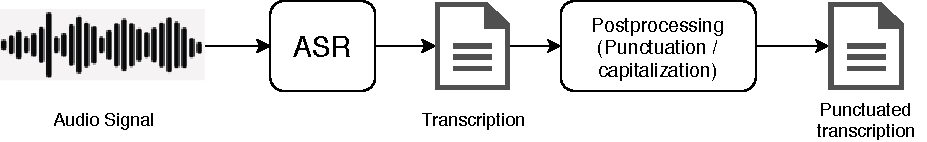
\includegraphics[width=\linewidth]{img/Punctuation_on_ASR_output.pdf}
  \caption{Punctuation and capitalization as a postprocessing step after ASR.}
  \label{sota:figure:punc_on_text}
\end{figure}

Punctuation using only textual features is relevant when e.g.~punctuation restoration is needed for written data \citep{jakubicek2010punctuation} or in the case when corresponding audio information is lost \citep{lu2010better}. In \cite{jakubicek2010punctuation}, for instance, the punctuation detection is addressed from a syntax-based perspective by using the output of an adapted chart parser, which provides information on the expected punctuation placement. In \cite{ueffing2013improved}, several textual features including language model scores, token n-grams, sentence length and syntactic information extracted from parse trees are combined using conditional random fields (CRF). They demonstrate that syntactic features help only when the input language is well-structured (as e.g.~newspaper texts). In \cite{lu2010better}, the task is based on dynamic CRF and applied to a conversational speech domain where sentence boundaries and types are detected. 

Another reason that facilitates the usage of solely textual features is the abundance of well-punctuated written data. Using a purely text-based n-gram language model, \cite{Gravano} demonstrate the performance improvement induced by large textual training in punctuation detection and capitalization. Although narrow-range grammatical constructions are recognized well for comma and period placement, n-gram approach fails in discovering long-range dependencies for the correct placement of question marks. 

Punctuation placement is also approached as a monolingual machine translation problem in \cite{peitz2011modeling, Cho2017NMTbasedSA, Paulik, Klejch} where target sequence is the punctuated version of the source sequence. 
  
Recently, usage of DNN-based systems has shown remarkable performance in the task for their ability to capture long-range dependencies in sequential data. These models use \textit{word embeddings} to represent words as vectors in a high-dimensional space that reflects their semantic, syntactic and morphological behaviour in the language \citep{mikolov_wordvec}. \cite{ballesterosneural} introduces a language-independent model with a transition-based algorithm using LSTM, without any additional syntactic features. \cite{Treviso} experiments with different word embeddings model within an RNN-based setup and proves that a good word embeddings model improves punctuation restoration accuracy. \cite{Che2016PunctuationPF} follows a convolutional neural network-based approach where the punctuation is predicted for the third word in a 5-word window and reports improvement on a similar non-DNN based approach that uses n-grams \citep{ueffing2013improved}. A task specific approach is followed in \cite{emrai} where punctuation marks are restored in medical dictation transcripts. They show that accuracy of state-of-the-art RNN-based methologies can be improved to a large extend using vocabulary reduction techniques adapting to the language domain. 

\subsection{Neural Machine Translation}
\label{sota:nmt}

Machine Translation is defined as the automatic conversion of a sequence of symbols in one language to a sequence of symbols in another language \citep{bengio_dl}. It has evolved through years from rule-based systems (RBMT) to statistical approaches (SMT), which modeled the probabilities of mappings between sub-phrases of various sizes. These probabilities are learned in a statistical fashion from \textit{parallel texts} where sentence aligned translations are available in the languages involved (referred as source and target languages). 

Neural machine translation (NMT) quickly replaced SMT in the recent years for its relatively simpler architecture and better performance. Usage of sequence-to-sequence architecture for this task was first introduced in \cite{sutskever} and made it to commercial spectrum in 2016 as the preferred architecture for the task \citep{google_nmt}. \textit{Transformer} architecture further simplified this model in and also recorded better performance \citep{transformer}.

%It no longer needed fine-tuning of smaller components involved in a SMT system and directly learned mapping from input text sequence to the target text sequence \citep{bahdanau, google_nmt}.

\begin{figure}[t]
  \centering
  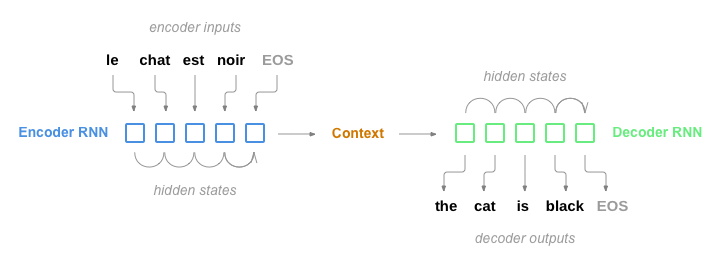
\includegraphics[width=\linewidth]{img/spro_nmt.png}
  \caption[Architecture of an encoder-decoder neural machine translation system.]{Architecture of an encoder-decoder neural machine translation system. (Diagram taken from \textit{spro}'s\protect\footnotemark sequence-to-sequence translation tutorial on github)}
  \label{sota:nmt_schema}
\end{figure}

\footnotetext{\url{https://github.com/spro}}

A commonly used architecture for NMT is the encoder-decoder architecture. As illustrated in Figure \ref{sota:nmt_schema}, token vector sequence in the source language input through an encoder is sent over to a decoder to output token vectors of the target language. Tokens can either represent words \citep{sutskever}, sub-word units \citep{google_nmt} or characters \citep{Ling2015CharacterbasedNM, marta}. Similar to the data-driven approach of SMT, this network is trained with parallel text, generally on sentence level, to maximize the probability of a correct translation given a source sentence \citep{bahdanau}.

\begin{figure}[t]
  \centering
  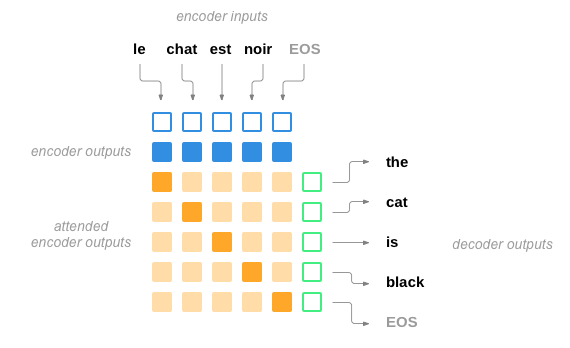
\includegraphics[width=0.8\linewidth]{img/spro_nmt_attention.png}
  \caption[Attention mechanism in encoder-decoder NMT architecture.]{Attention mechanism in encoder-decoder NMT architecture keeps track of portions of the input sequence that affects each decoder output. (Diagram taken from \textit{spro}'s sequence-to-sequence translation tutorial on github)}
  \label{sota:nmt_attention}
\end{figure}

One weakness that this model introduces is the connection between two RNNs that squeezes the input sequence into one single-length vector before being decoded as target token sequence. This is analogous to reading a phrase from beginning to end and then translating it into another language without looking at it again. Normally, a translator would break a input sentence into smaller portions and translate step by step giving attention to a different parts each time. An analogy of this approach was implemented in NMT with the introduction of \textit{attention mechanism} \citep{bahdanau, luong}. As illustrated in Figure \ref{sota:nmt_attention}, the attention mechanism helps focus on different parts of the input at each step of decoding. This relieves the decoder from having to predict target language tokens in one go without any spacial context of the input phrase \citep{google_nmt}. 

\textbf{Spoken language machine translation} is a type of MT where input and/or output to the system is spoken language. Spoken input translation can be employed through the usage of ASR prior to MT and translation can be generated as speech with a TTS to obtain spoken output. 

Machine translation with spoken input introduces its own specific challenges. First is that written and spoken domain show differences which could lead to degradation of performance if data domains are not compatible \citep{britz}. 

\begin{figure}[t]
  \centering
  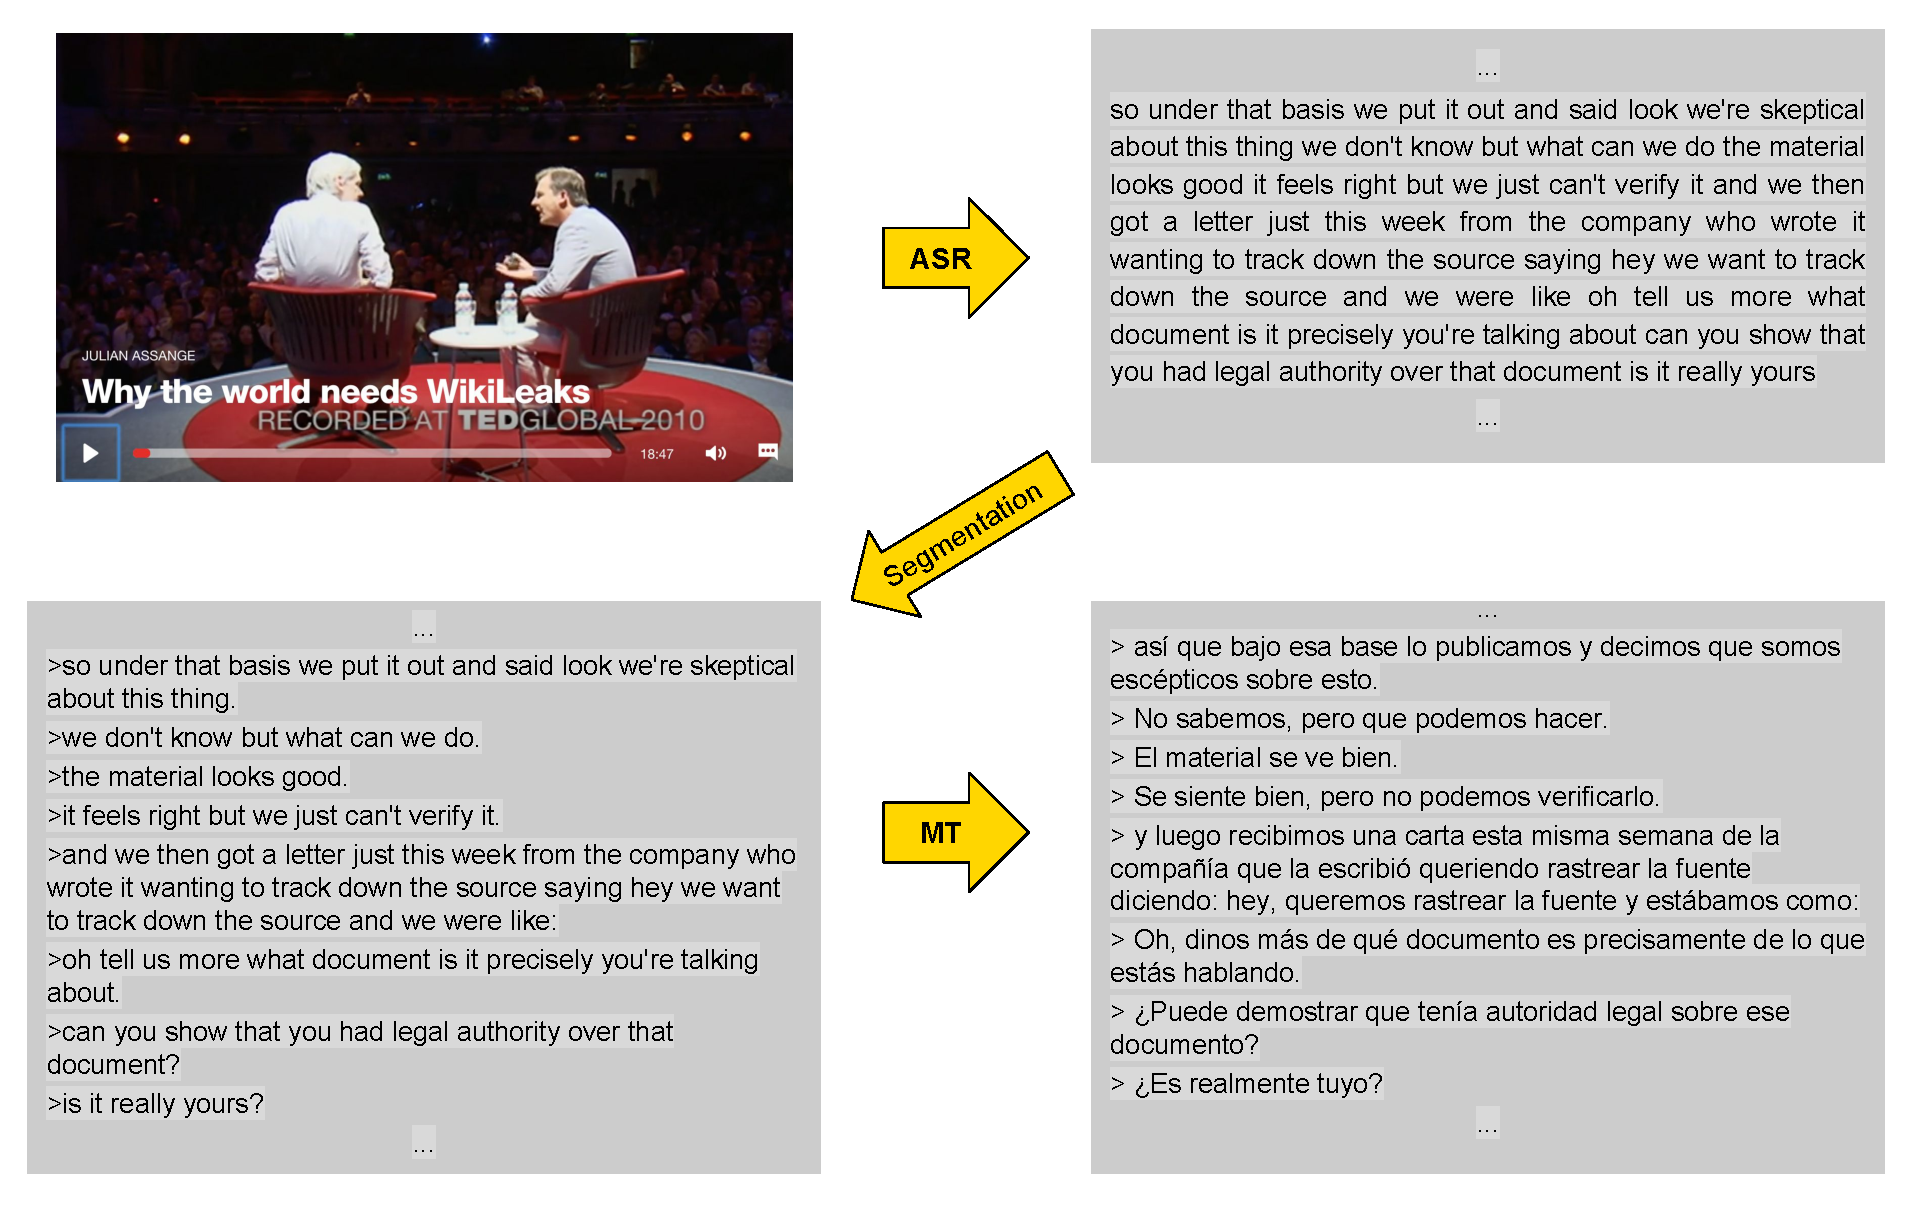
\includegraphics[width=\linewidth]{img/slmt_on_ted.pdf}
  \caption{Spoken language translation demonstrated on a conference recording.}
  \label{sota:tv_transcription}
\end{figure}

Another challenge that spoken language translation introduces is the possible incompatibility between ASR output structure and MT input structure. MT models are usually trained with sentence-like structures as samples and therefore show low performance on partial sentence or long sequences of words as input \citep{niehues2018}. In text translation domain, processing of long text documents is performed by translating it sentence by sentence using punctuation information as segmentation cues. A similar approach needs to be followed when input is spoken utterances as well. Figure \ref{sota:tv_transcription} illustrates an example of spoken language translation of a conference talk. A standard MT system would be unable to translate the unsegmented transcription of the talk. Translation is made possible only through a segmentation process, such as boundary detection or punctuation restoration. 

A topic worth mentioning in the area of translation is methods for measuring the accuracy of automatic machine translation methods. Commonly used metrics like \textit{BLEU} offer a remedy for the expensive labour involved in human evaluation of translation. The evaluation is performed in comparison with human translations. Given a testing set, each machine translated sample is compared to a reference translation and given a score of how close they are. \textit{BLEU} that stands for \textit{Bilingual Evaluation Understudy} measures this by calculating the ratio of matching n-grams in the translation and reference text \citep{bleu}. A BLEU score is basically a number between $0$ and $1$, $1$ signifying a higher similarity between the texts. The quality of a MT system is usually estimated with an average score among a set of testing samples and reported in percentage. 

\subsection{Text-to-Speech Synthesis}
\label{sota:tts}

%TTS:concatenative TTS
Speech synthesis involves production of a human-like speech given a text input with computational methods. Before the advent of deep learning, there were two main approaches to text-to-speech (TTS) synthesis: concatenative TTS, and parametric TTS. Concatenative TTS, also called unit selection, combines short pre-recorded audio clips called units to synthesize the desired text \citep{vanSanten:1997:PSS:241679}. Figure \ref{sota:figure:concatenative_tts} illustrates this process. A linguistic analysis performed on the text dictates which units to be selected in which order to form the waveform from an audio codebook consisting of phones, biphones or triphones. Since audio units are based on real speech samples, this technique can provide a good performance in terms of speech quality. That is, it sounds very similar to real human speech. However, the cut and stitch procedure involved often results in lack of naturalness. Also, this technique proves to be less flexible since its construction involves creation of a carefully designed large database. 

\begin{figure}[t]
  \centering
  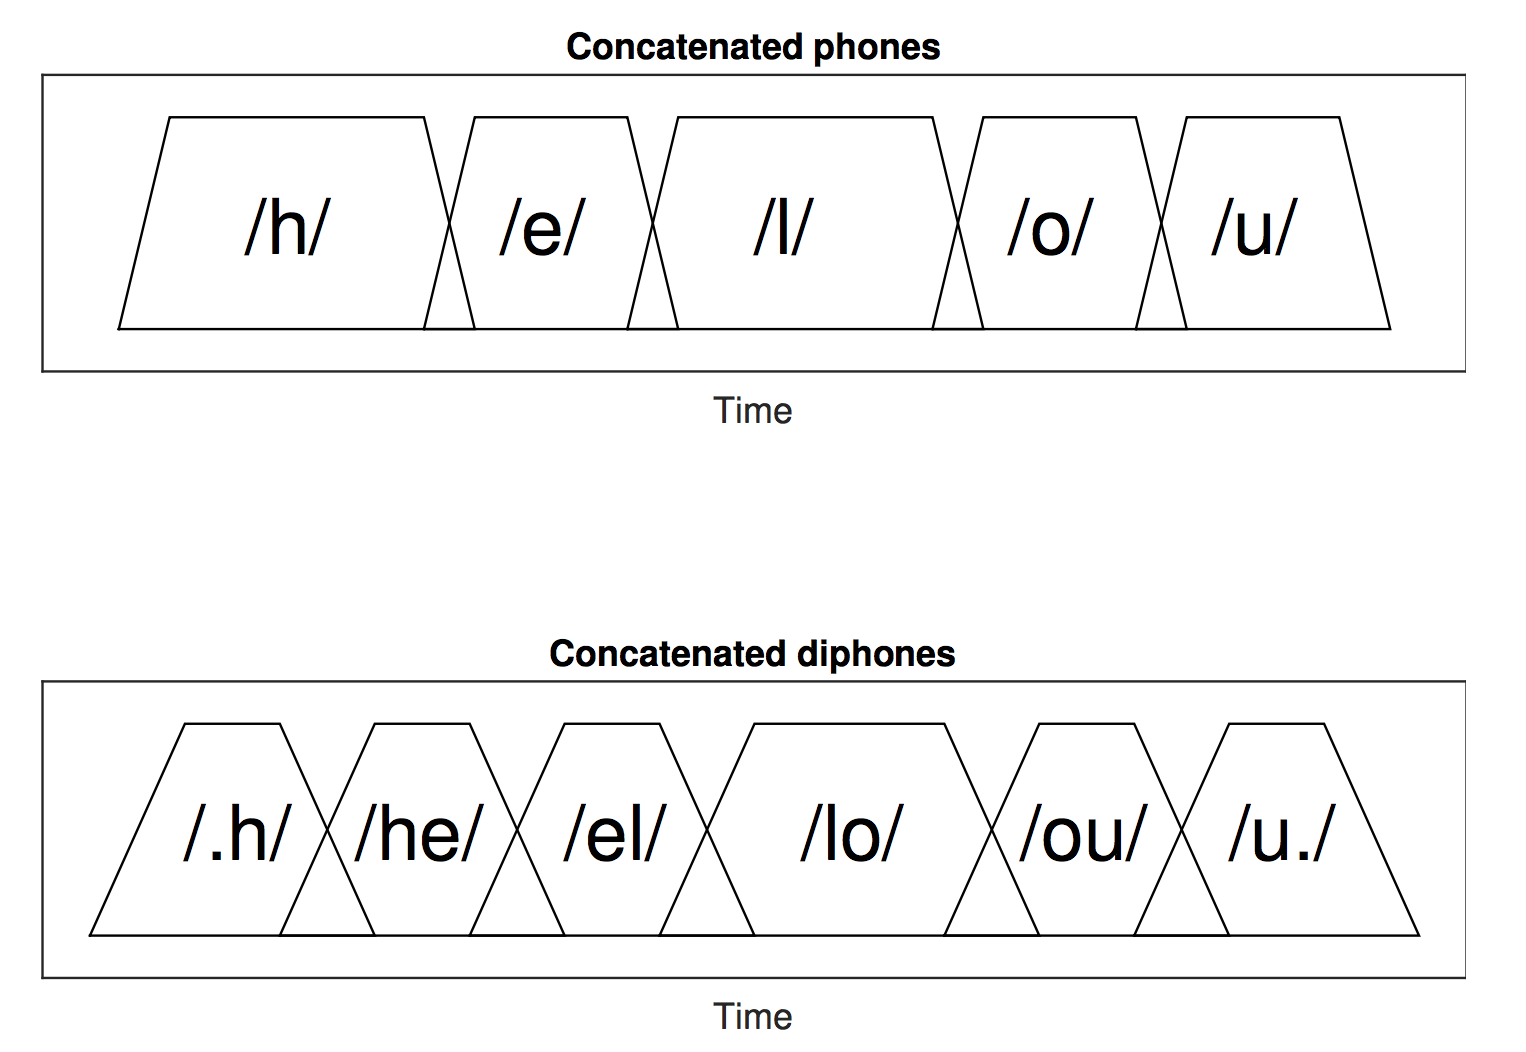
\includegraphics[width=0.7\linewidth]{img/concatenative_tts.png}
  \caption[Speech synthesis from units in concatenative TTS.]{Speech synthesis from units in concatenative TTS. (Credit: Tom Bäckström, Speech Synthesis Overview\protect\footnotemark)}
  \label{sota:figure:concatenative_tts}
\end{figure}

\footnotetext{\url{https://mycourses.aalto.fi}}

%parametric TTS
In contrast to having a large codebook, parametric TTS relies on statistical methods by generating speech with a combination of parameters like F0 and energy, modelling the human speech production \citep{Zen:2009:RSP:1576860.1577027}. Figure \ref{sota:figure:tts} illustrates the workflow of a parametric TTS system. First, morphemes in the input text are converted to phonemes through a linguistic analysis. Next, features like cepstra, F0, duration and break are calculated to be fed into the \textit{vocoder}. The vocoder finally generates the waveform using these parameters. The parameter probabilities is learned from phonetically labeled speech data and modeled as Hidden Markov Models (HMM). Recently introduced DNN-based models follow a similar approach but replace the HMM-based modelling with DNN \citep{zen_dnn}. End-to-end models, on the other hand, employ a DNN to directly synthesize speech from characters \cite{Wang2017}.

\begin{figure}[t]
  \centering
  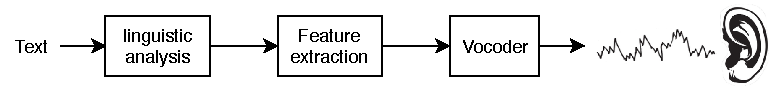
\includegraphics[width=0.9\linewidth]{img/tts_diagram.pdf}
  \caption{Basic workflow of a statistical text-to-speech system.}
  \label{sota:figure:tts}
\end{figure}

%Prosodic modelling
There exist two main parameters in evaluating a TTS system: intelligibility and naturalness. Intelligibility, as its name suggests, measures to what extend the linguistic information in a synthesized speech waveform can be comprehended. Naturalness, on the other hand, deals more with the way how an utterance is said and measures roughly the likelihood that it was said by a person and not a machine \citep{naturalness}. Naturalness is almost directly related to the prosody production in a TTS system. Prosody modelling in a TTS is predicted in three dimensions which are intonation, duration and breaks. Among a few theories on intonation modelling are the \textit{Fujisaki model} \citep{Fujisaki1983}, \textit{Tilt model} \citep{tilt}, \textit{Bezier polynomial coefficients} \citep{Escudero2002}, and \textit{Tones and Break Indices (ToBI)} \citep{tobi, Pierrehumbert}. Duration modelling deals with the prediction of segment (phone or syllable) lengths in speech. Breaks also have an important role in achieving naturalness in speech as it helps structure the discourse and also occur naturally from respiration. They can be manifested in two ways: silent, or filled, i.e.~through lengthenings or filler words \citep{zellner}. Several approaches exist for break prediction in TTS. Some recent works include \cite{DBLP:journals/pdln/AgueroB03} which models disfluency in synthesized speech through filled pauses to mimic a talking-style speech opposed to the a reading-style. \cite{DBLP:conf/iberspeech/PascualB16} focuses on silent break detection by employing RNNs. 

\subsubsection*{External Prosodic Encoding to TTS}

Some implementations of TTS systems allow the taking of external labels to influence the prosodic parameter selection process. This is performed through an interface called \textit{markup language} which accompanies the text input and conditions the sythesized speech on various acoustic/prosodic aspects. One well-known implementation of this interface is \textit{Speech Synthesis Markup Language (SSML)} \citep{ssml}. An example of an input segment to a state-of-the-art TTS system\footnote{\textit{IBM Watson TTS}: \url{https://text-to-speech-demo.ng.bluemix.net/}} that utilizes SSML tags is given below.

\begin{lstlisting}
<p><s>Conscious of its spiritual and moral heritage <break time="300ms"/>, the Union is founded on the indivisible, universal values of <prosody rate="-15%">human dignity, freedom, equality and solidarity.</prosody> It is based on the principles of democracy and the rule of law <break time="500ms"/>. </s> <s> It places the individual at the heart of its activities, <prosody rate="+15%">by establishing the citizenship of the Union</prosody> and by creating an area of freedom, security and justice.</s></p>
\end{lstlisting}


The synthesis is indicated on where to break for how long using the tag \textit{break} and tuned to speak faster or slower with the tag \textit{rate}. Usually, tags that are related with pitch, speech rate and volume are set with relative percentages and have an estimated effect on the outcome instead of an absolute effect. 

\subsection{Speech-to-Speech Translation}
\label{sota:s2s}

\begin{figure}[t]
  \centering
  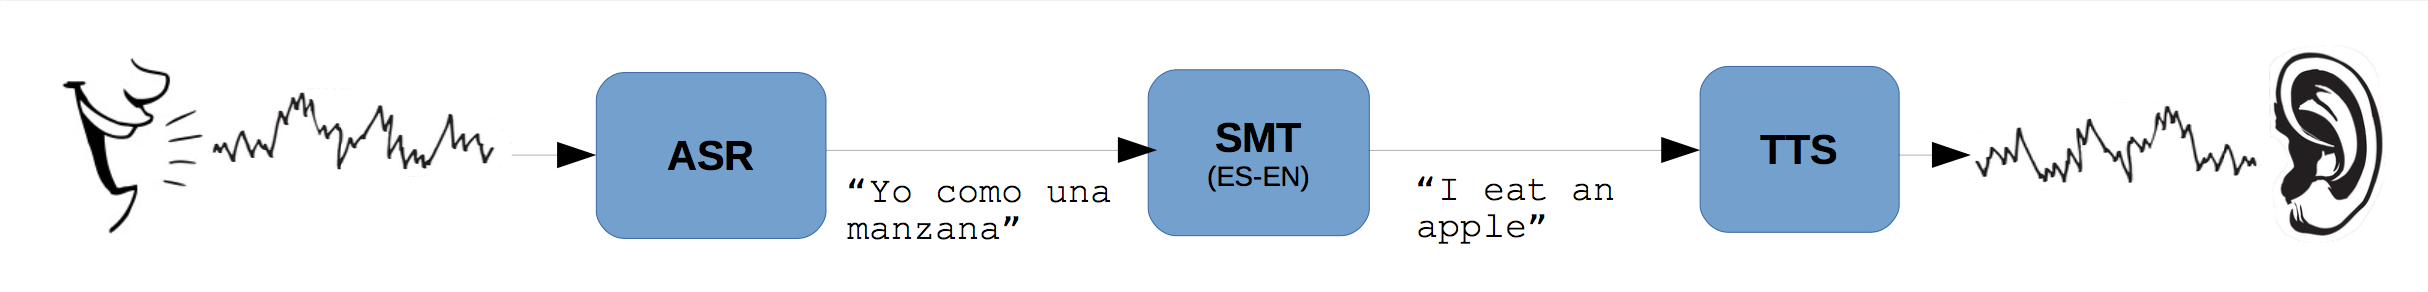
\includegraphics[width=\linewidth]{img/s2s_classic_pipeline.png}
  \caption{A conventional speech-to-speech translation pipeline.}
  \label{sota:s2s_classic}
\end{figure}

Speech-to-speech (S2S) translation enables human-to-human communication where each of the agents involved speaks in a different language. A device capable of enabling such a communication is able to accept spoken input in language A, translate it to language B and then synthesize it for hearing. By performing this process in both ways, it acts as an interface for a turn-based inter-lingual communication. Conceptually, such a system is the concatenation of the three following processes: (1) ASR, (2) MT, and (3) TTS. A diagram of the one-way process in S2S translation is illustrated in Figure \ref{sota:s2s_classic}. 

There exist various examples of S2S translation solutions resulting from both academic and commercial research. \textit{Verbmobil} is considered as the pioneer in the field as it is the oldest and most extensive research project dealing with S2S translation \citep{wahlster2013verbmobil}. It was designed for translation of spontaneous dialogues in mobile situations for the languages English, German and Japanese. \textit{IBM MASTOR} was developed in a defense oriented framework for facilitating spoken communication in low-resource languages \citep{ibm_mastor}. European Union funded project \textit{TC-STAR} was the first that addressed S2S translation in an unrestricted domain between languages English, Chinese and Spanish \citep{tcstar}. Its local counterpart \textit{TECNOPARLA} was developed with the motivation of spoken translation in the broadcast radio and television domain for the languages Catalan, English and Spanish \citep{tecnoparla}. \textit{EMIME} project was the first work that aimed voice personalization through S2S translation, where synthesized voice is adapted to sound like the recognized voice \citep{emimeemime}. Two projects with Swiss origin, \textit{SP2 SCOPES} \citep{sp2} and \textit{SIWIS} \citep{Garner:199815} that focus on Swiss and Eastern European languages report cross-lingual prosodic transfer as their main objectives. Although, there are no recorded results on the accomplishment of these objectives. 

\subsubsection{Spoken Parallel Corpora}

\begin{table*}[ht]
\begin{center}
\begin{tabular}{>{\arraybackslash} m{0.42\linewidth} >{\arraybackslash} m{0.21\linewidth} >{\arraybackslash} m{0.3\linewidth}}
\bf Corpus & \bf Languages & \bf Speech style \\ \toprule
EPIC                                            & en/it/es              & spontaneous/interpreted   \\
TC-STAR                                         & en/es, en/zh          & spontaneous/interpreted   \\
MSLT                                            & en/fr/de              & constrained \\
EMIME                                           & fi/en, de/en          & prompted                  \\
EMIME Mandarin                                  & zh/en                & prompted                  \\
SP2-Speech-Corpus                               & en/fr/de/hu/mk/sr     & prompted w/ emphasis    \\
Japanese-English emphasis                       & ja/en                & prompted w/ emphasis    \\
SIWIS database                                  & en/fr/de/it           & prompted w/ emphasis    \\
MDA~\citep{almeman2013multi}                    & 4 Arab dialects  & prompted                  \\
Farsi-English~\citep{Melvin2004CreationOA}      & fa/en                 & read/semi-spontaneous     \\
\bottomrule
\end{tabular}
\end{center}
\caption{\label{sota:corpora} A selection of available parallel speech corpora for use in S2S translation. }
\end{table*}

%Why spoken parallel corpora needed intro
The availability of large parallel corpora is one of the major challenges in developing machine translation systems. Bilingual corpora, which are needed to train statistical translation models, are harder to acquire than monolingual corpora since they presuppose the implication of labour in translation or interpretation. Working on the speech domain introduces even more difficulties since interpretations are not sufficient in capturing the paralinguistic aspects of speech. The profession of interpretation aims rapid spoken translation of speeches in e.g.~conferences, diplomatic gatherings and do not give any attention to the re-enacting of any paralinguistic features. In contrast, dubbing also covers for this aspect since the aim is to have translated voice segments of a movie or series that match with the context and lip movements in the original language. Although this domain could be rich for obtaining expressive parallel corpora, it has not been explored in any previous work. In Chapter \ref{chapter:corpusWorks}, I will explain my work in detail dealing with this type of domain \citep{bucc, Oktem2018}.

Several attempts have been made to compile large spoken parallel corpora from interpreted or fully-prompted material. Some of these corpora that were published in literature are listed in Table~\ref{sota:corpora}. Each of them show some differences in terms of its source and the way translation was handled. The EPIC corpus has been compiled from speeches from the European Parliament and their interpretations \citep{bendazzoli2005approach}. The 1 hour voice conversion corpus collected within the TC-STAR project also contains speech segments from the European Parliament and their interpreted versions in Chinese and Spanish \citep{tcstar_corpora}. The EMIME database is a compilation of prompted speeches to serve for the task of speaker conversion \citep{wester2010emime}. The MSLT corpus has been collected in bilingual conversation settings, but `there is no one-to-one alignment between sentences in the different languages as they are lightly guided conversations \citep{federmann2016microsoft}. There is a number of corpora collected for projects focusing on the emphasis translation task: SP2 Speech Corpus \citep{sevcujski2016design}, SIWIS database \citep{siwis_db} and the database collected by \cite{quoc_corpus}. These corpora contain sentence recordings with acted emphasis on the same word or word groups in both languages. 

\section{Speech Prosody Overview}
\label{sota:prosody}
In this section I will try to break down prosody to get an overview on its role in speech and also its characteristics. According to the definition by \cite{Fujisaki97}, role of prosody in speech is to organize linguistic units into an utterance and its realization involves segmental and suprasegmental features of speech. What is referred to as segmentals in this expression are the phonemes, syllables and words that have distinct boundaries in the utterance. On the other hand, suprasegmentals refers to the elements that can span over or partially cover segments in speech \citep{palmer}. Suprasegmental features in speech are the following prosodic elements: intonation, rhythm and stress. These features can be briefly explained as:

\begin{itemize}
    \item \textbf{Intonation} deals with the melodic aspects of the speech, and is realized by pitch movements. Pitch is what is perceived through the fundamental frequency (F0) involved in an audio signal. 
    \item \textbf{Rhythm} deals with the timing of phonemes, syllables and pauses in speech. Speech rate, which gives the number of segments uttered in a unit of time, is also a feature derived from rhythm.
    \item \textbf{Stress} deals with the energy in speech and is perceived through the speech signal amplitude. 
\end{itemize}

Figure \ref{sota:figure:prosodicfeatures} shows visualization of a short speech segment on Praat where pitch contour and intensity can be visualized over word and phoneme segments.  

Prosodic features are employed in speech in a complex manner to convey linguistic, para-linguistic and non-linguistic information \citep{Fujisaki97}. I will try to demonstrate the uses of these features on some examples in English. 

Intonation is considered as one of the key features in conveying attitude in many languages \citep{Prieto}. Prieto gives the simple sentence \textit{``I am cold.''} as an example for this. With different intonation structures this sentence could have many different meanings including contradiction, command (as a request to close the window) and surprise. Intonation can also be used to mark modality in sentences.  Yes/no questions, for example, commonly end with a rising pitch in English. 

Stress feature is used for marking salient points in discourse or to encode givenness. Take the example \textit{``The butler killed the him.''}. A word is marked with a stress depending on which element is already mentioned and which element is new information. This type of encoding can also be defined as phrasal stress or accent.

Rhythm and pausing is relevant in forming a hierarchical organization in speech through phrasing. The example given in \cite{zellner} expresses this very well. The length of the inter-lexical pause in \textit{``a Turkish carpet salesman''} can help distinguish if the carpets or the salesman is Turkish. Audio waveforms of both versions are visualized in the Figure \ref{sota:figure:carpet}.

\begin{figure}[t]
  \centering
  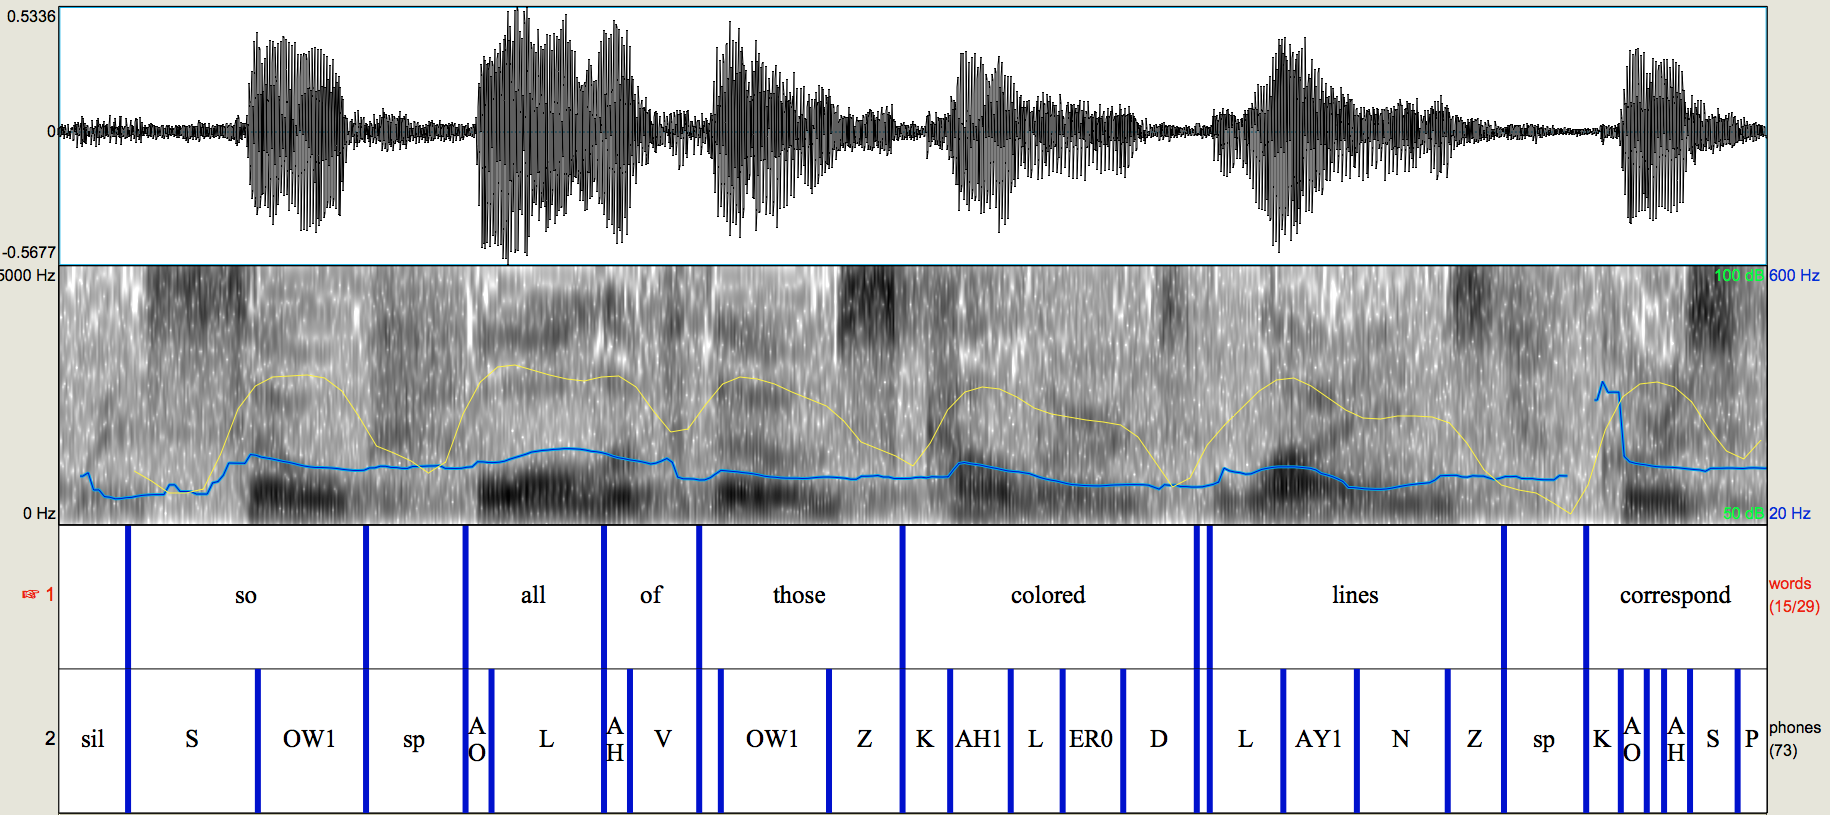
\includegraphics[width=\linewidth]{img/prosfeats_praat.png}
  \caption{Segmental (phoneme and word) and suprasegmental (pitch in blue, intensity in yellow) features of a speech signal shown with the audio waveform and frequency spectrogram. }
  \label{sota:figure:prosodicfeatures}
\end{figure}

\begin{figure}[t]
  \centering
  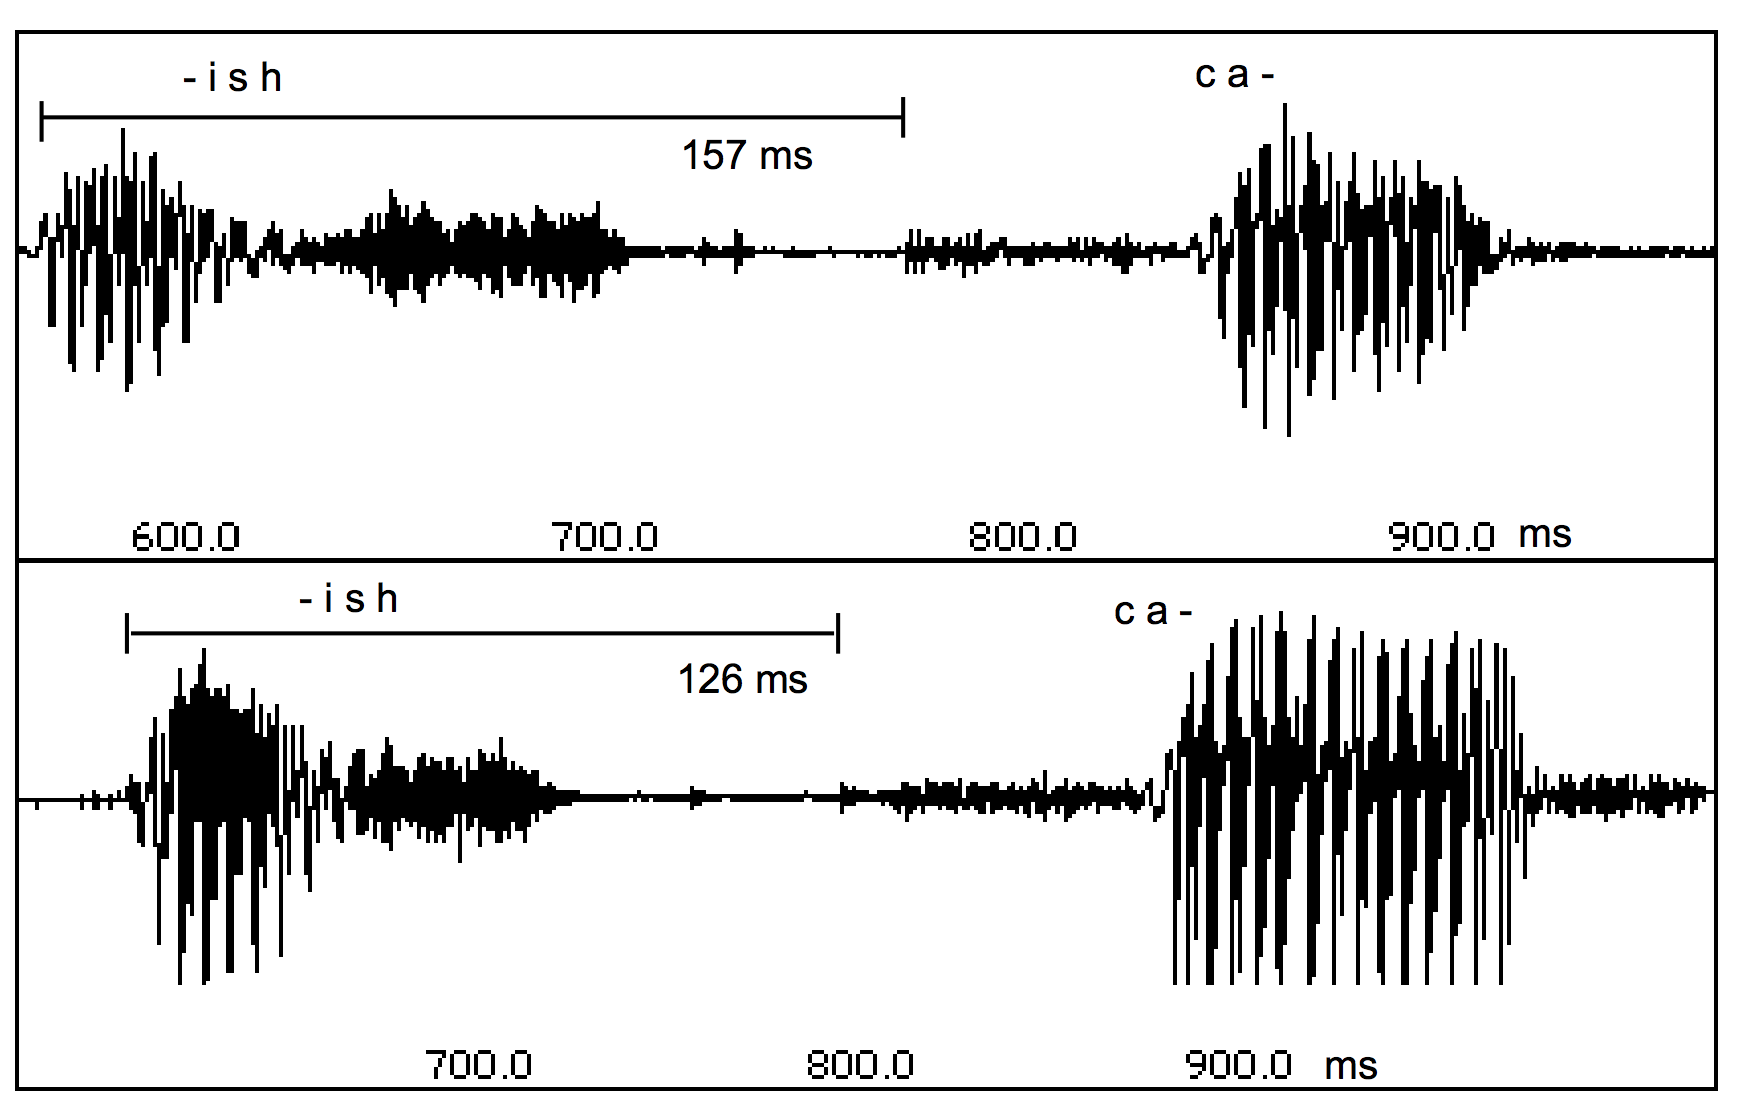
\includegraphics[width=0.8\linewidth]{img/carpet.png}
  \caption[Phrasing in speech affecting meaning.]{Phrasing in speech affecting meaning. Above ``a Turkish (carpet salesman)'', below ``a (Turkish carpet) salesman''. (Example and figure taken from \cite{zellner})}
  \label{sota:figure:carpet}
\end{figure}

It has to be noted that use of prosodic elements vary greatly between languages. In tonal languages like Chinese, Somali or Thai, it is used for encoding different semantics of words. In intonational languages like Spanish and Catalan, position of the word accent also can infer different meanings. 

Prosody is also realized in the para-linguistics of speech such as emotional state and attitude. These features however, tend to show more variety between different languages, cultures and classes \citep{cowie}. 


\section{Prosody in Speech Processing}
In Section \ref{sota:neuralspeech} I gave a review of the systems where spoken language is being processed to serve for a certain purpose. However, in these systems, speech is considered only with the linguistic content (i.e. words, phrases, etc.) it carries. Prosodic features that are encoded through various acoustic phenomena like intonation, energy, breaks etc. are disregarded in any further analysis.  

In this section, I will review recent as well as some historical works that regard prosody as an essential dimension in a speech processing framework. These works not only argue that prosodic features in spoken language are important for spoken language applications, but also suggest methodologies for their inclusion and report progress through it. 

I will present two applied areas where prosodic cues are utilized as an advancement for speech processing systems. First, in automated speech transcription where prosodic cues are used for phrase boundary detection or punctuation restoration, then in speech-to-speech translation where a complete linguistic and paralinguistic information transfer is desired.

\subsection{Utilizing Prosody in Punctuation Restoration in Transcribed Speech}
\label{sota:punk_prosody}
It has been shown that prosodic features are highly indicative of phrase boundaries as well as of punctuation placement in many works \citep{punctuation_book}. Therefore, a great deal of effort has been put in several works into the use of prosodic features in punctuation restoration when original speech is available. In \cite{levy2012effect}, the authors successfully detect automatically full stops in ASR output with no language modeling using only weighted pause, F0 changes and amplitude range values. Commas are shown to be more difficult to detect when only prosodic features are used. In \cite{baron2002automatic}, it is demonstrated that combination of language and prosodic models performs better than single-model approaches. 

Many studies consider punctuation restoration as a problem of determining the probability of a certain label at a boundary point in speech, e.g. between words or at pauses, calculated in the vicinity of that point. Prosodic and textual cues around each inter-word boundary are taken as features for a decision tree classifier to detect sentence boundaries in \cite{liu2006study}. Similarly in \cite{khomitsevich2015combining}, word and grammatical n-gram features are combined with prosodic features to detect punctuation marks in Russian ASR system. \cite{Psutka04automaticpunctuation} focus on Czech broadcast news speech to detect commas and sentence boundaries by using a prosodic model based on decision trees and language model based on n-grams. 

A combination of lexical-, prosodic-, and speaker-based features is also found in \cite{batista2012bilingual} for the detection of full stops, commas, and question marks in a bilingual English-Portuguese broadcast news corpus. Similar works deal with the punctuation generation problem by using statistical models of prosodic features \citep{Christensen01punctuationannotation}, the combination of both textual and prosodic features based on adaptive boosting \citep{kolar2012development}, and a cross-linguistic study of prosodic features through two different approaches for feature selection: a forward search wrapper and feature filtering \citep{fung2007cross}. Also, in \cite{Klejch}, frame-level prosodic features (only pitch and pause) are integrated in a neural machine translation based system with a hierarchical encoder.

Combining lexical and prosodic models has been employed in a bidirectional neural network setting in \cite{Xu2017} for sentence boundary detection and in \cite{tilk2016bidirectional} for punctuation restoration. Both approaches are based on training of the language model (on large amounts of textual data) separately to the acoustic model (from a smaller corpus), eventually leading the models to bias on written data. 

\subsection{Utilizing Prosody in Spoken Language Machine Translation}
\label{sota:prosody_in_smt}

% Utilization prosody is relevant in SLMT in three ways: (1) for segmenting input into sentence-like units (2) for  it can be helpful in resolving ambiguous translations and (2) it is worth to carry prosodic features to the target synthesis on a S2S translation setup. 

% The example given earlier from \cite{zellner} is helpful in demonstrating the use of prosody in a spoken language input translation system. The phrase ``Turkish carpet salesman'' could be translated in two ways to Spanish: either ``vendedor turco de alfombras'' or ``vendedor de alfombras turcas''. This disambiguation is only possible through the perception of the break and intonational structure in the sentence. 

%intro
There has been considerable work on inclusion of prosody into speech-to-speech translation pipelines. Most of the research based systems give some of the focus onto this area as it is believed that spoken translation is truly complete only through conveying of prosody as well as linguistic information between source and target phrases. On another aspect, some research focus on the fact that ASR output is not optimized to be inputted to machine translation. ASR outputs only a raw sequence of words without any further information on sentence or phrase boundaries and thus harms MT quality that necessitates a certain input size and context. 

It is observed that there are three main objectives when it comes to incorporation of prosody into a S2S framework. These objectives are: (1) segmentation of the source phrase into meaningful units through use of prosody to aid the machine translation step, (2) transfer of prominence (emphasis) in input speech into the synthesized translations and (3) using context information to boost translation accuracy. 

%first use verbmobil (2000)
First use of prosody within a spoken language translation system was within the \textit{Verbmobil} project \citep{verbmobil_prosody}. A group of prosodic features were computed for the word hypotheses computed by the ASR module. These were: probabilities for clause boundaries, accentuation and sentence mood. Among these, a major improvement was achieved through the classification of clause boundaries in the input phrases. Syntactic parsing of the recognized words was improved in terms of readings and computation time only through the segmentation of the input phrases. Boundary classification was based on a combination of textual and prosodic features (energy, duration and F0). A similar approach is investigated in \cite{Matusov07improvingspeech}. A lexical-prosodic boundary prediction algorithm is introduced and compared with various other segmentation algorithms in terms of their effect on translation quality. They show that translation is optimized through usage of a boundary prediction algorithm based on prosodic features and phrase probabilities using a language model. 

%aguero, adell, bonafonte
\cite{aguero2006prosody} can be considered as the first example where objective is to transfer the underlying paralinguistic features in the source speech to the synthesized target speech. The methodology they present aims to find transfer patterns of F0 contours in source and target speech in a S2S framework. This is done with an extension on the intonation prediction module of the TTS that does not only consider linguistic features of the target translation but also features derived from the source speech. The intonation patterns of phrases of the input sentence is first classified and then mapped into intonation patterns of the target language. These transformations are learned from a bilingual corpus and integrated as an enhancement to a phrase-based translation system. They report improvement over preferences of the synthesized translations in terms of naturalness. 

%CSU
A similar approach is followed in \cite{anumanchipalli:2012} for word-level emphasis transfer. They explain their motivation with experimentation on a subset of the bilingual speech corpus they collected. By manual inspection, they see that there's a match of 48\% of the emphasized words in the parallel languages. Their cross-lingual intonation transformation methodology is based on learning the mapping between word-level intonation contour parametrizations between two languages from a single-speaker bilingual dataset. Since they do not perform the machine translation itself, they are able to compare intonation contours generated in a neutral way and with their enhancement. They show that through this process generated contours get closer to the reference contours in their dataset.

%TODO: \mireia{Here I miss some more recent works on emphasis transferring that we found last year, like Honnet's thesis: \footnote{http://publications.idiap.ch/downloads/papers/2017/Honnet_THESIS_2017.pdf} %http://publications.idiap.ch/downloads/papers/2017/Honnet_THESIS_2017.pdf}

Do et al.~approach cross-lingual prosodic transfer from a perspective based on transferring of word-level emphasis. Their general approach is to label each word in the source token sequence with a real-numbered emphasis level and then map it into the words in target sequence using a transformation function. Emphasis modelling is performed with linear-regression hidden-semi Markov models (LR-HSMMs) that is trained on F0, duration and energy features \citep{Quoc2016}. Their methodology for mapping input emphasis estimations to target emphasis weights show change over various works. In \cite{Quoc2016}, this is performed using a model based on conditional random fields (CRFs) (Figure \ref{sota:quoc}a). Following, in \cite{Quoc2016b}, they utilize a LSTM based model with attention that exploits the word alignment information of machine translation. They record an improvement of 1\% in terms of emphasis prediction F-measure (Figure \ref{sota:quoc}b). Both of these approaches incorporate prosodic transfer process as an additional module besides MT and assume perfect translations. This is later addressed in \cite{Quoc2017} and \cite{Quoc2018} where emphasis and word prediction are done jointly within a sequence-to-sequence MT system (Figure \ref{sota:quoc}c). The lack of parallel spoken data is covered by a two-stage training procedure. Translation model is first trained on a large text corpus and then emphasis modelling is generated from a smaller laboratory generated English-Japanese parallel corpus. Their results show that text translation does not improve with inclusion of emphasis weights. As a simpler system is introduced, gain on computational time is recorded, however, without an improvement on emphasis prediction compared to previous works. All in all, they report that their models are speaker dependent and is demonstrated on a highly controlled setting. This can be explained by the corpus they use at hand which consists of a small set of samples with acted emphasis. 

\begin{figure}
\centering
\begin{tabular}{c}
  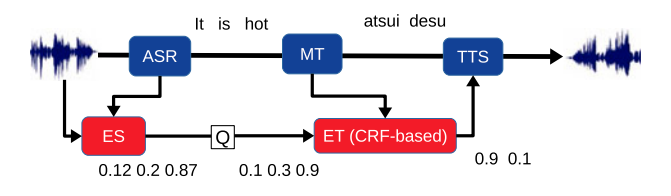
\includegraphics[width=0.7\linewidth]{img/quoc_a.png} \\
(a) CRF-based \\[6pt]
 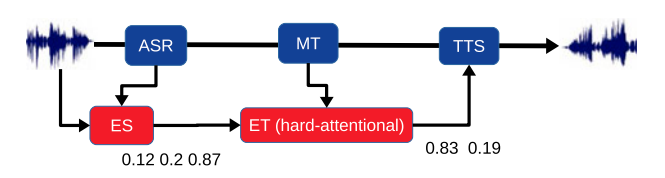
\includegraphics[width=0.7\linewidth]{img/quoc_b.png} \\
(b) Hard-attentional \\[6pt]
 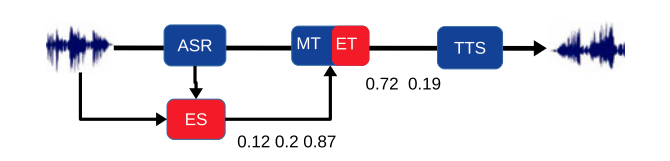
\includegraphics[width=0.7\linewidth]{img/quoc_c.png} \\
(c) Joint model \\[6pt]
\end{tabular}
\caption[Various implementations of S2S translation systems with emphasis transfer.]{Various implementations of S2S translation systems with emphasis transfer. (Diagrams are taken from \cite{Quoc2018}) }
\label{sota:quoc}
\end{figure}

%pause transfer
Pausing in speech is an important prosodic feature that affects both emphasis perception and phrasing. Transfer of pauses within S2S translation is addressed in the works: \cite{truong2015_iwslt} and \cite{bonafonte:pausetransfer}. In the former one, pause prediction is incorporated into the CRF-based emphasis prediction module and shows improvement in terms of emphasis perception in the synthesized examples. The latter work focuses on the transfer of the phrasing and follows a rule-based approach exploiting alignment information from SMT. 

%context enrichment
Some work on use of prosody in S2S translation focuses on employing prosodic features available through acoustic or linguistic analysis to further boost translation accuracy. These works are mostly inspired from approaches where factored SMT is enhanced with linguistic features (e.g.~POS features) and employ a similar approach in spoken translation. \cite{Guo2016} is an example where additional prosodic features based on pronunciation, boundary marks and emphasis is integrated as factors to a factored translation model based system. They record slight improvement in terms of translation accuracy with inclusion of boundary marks when translated from Chinese to English. In the opposite direction, they record improvement with inclusion of all three features. Again in \cite{RangarajanSridhar:2013:enrichingS2S}, factored translation models used for phrase-based translation is extended to accept additional prosodic information on source and target sides. They test inclusion of dialog information such as question types in source side and pitch accent based prominence features on the target side. Modest improvements are recorded in terms of translation accuracy. 

Having reviewed the fundamental concepts and state-of-the-art, I will move in next section on presenting the corpus related work. 